\section{Auswertung}
\subsection{Datenaufbereitung}
Ein bereitgestelltes $C++$ Programm wählt nur Daten aus, bei denen kontinuierliche Signale in den Layern auftreten und ordnet die verschiedenen Events in Zerfälle nach oben und unten

\begin{figure}[h]
	\includegraphics[width=140mm]{Aufbau}
	\caption{(a) \itshape Aufbau des Detektors: schwarze Balken symbolisieren Szintillatoren und schraffierte Flächen Metallplatten; (b) Ausrichtung der Spulen zur Erzeugung eines homogenen Magnetfeldes}
	\label{fig:Abbildung 1}
\end{figure}


\noindent und erstellt Histogramme. Zusätzlich müssen noch Korrekturen durchgeführt werden, da systematische Fehler wie Nachpulse und Detektorineffizienzen auftreten. Das Nachpulsspektrum wird dann mit einem Skalierungsfaktor statistisch gewichtet und vom Zerfallsspektrum subtrahiert. Für Zerfälle nach unten und oben gibt es verschiedene Skalierungsfaktoren $s_{up}$ und $s_{down}$. Ein Nachpuls wird nämlich nur für einen Zerfall nach unten gehalten, wenn der zugehörige Szintillator in diesem Moment ein Myon nicht detektiert hat und somit wird, um $s_{down}$ zu erhalten, $s_{up}$ noch mit der Ineffizienz der einzelnen Szintillatoren ($\leq 5\% $) multipliziert. Insgesamt sind also die Zerfälle nach unten deutlich weniger durch Nachpulse verfälscht.
\subsection{Bestimmung der Lebensdauer aus Messung ohne Magnetfeld}
Es wird ein Histogramm erstellt, in dem die Anzahl der Zerfälle aus allen Szintillatoren kombiniert gegen die Zeit aufgetragen wird. An diese Daten wird dann die Funktion \ref{eq:7} gefittet (Abbildung \ref{fig:Abbildung 2}). Das Verhältnis $f=\frac{N_0(\mu ^{+})}{N_0(\mu ^{-})}$ ist als $f = 1,275 \pm 0,05$ gegeben. Zum Abschätzen des systematischen Fehlers wird $f$ um $1\sigma$ bzw. $2\sigma$ variiert, sowie die Skalierungsfaktoren um $\pm 5\%$, und der Einfluss auf den Fit betrachtet. Man erhält durch quadratisches Addieren beider Abschätzungen $\Delta \tau _{0,sys} = 24.36 ns$ und $\Delta \tau _{C,sys} = 79.11 ns$. Durch das Variieren der Fitrange um $\pm 10 \%$ wird ein gegenüber s und f vernachlässigbarer systematische Fehler von $\Delta \tau _{0,sys,range} = 3.5 ns$ und $\Delta \tau _{C,sys,range} = 0.2 ns$ abgeschätzt.
Als Ergebnisse erhalten wir $\tau _0 = (2229\pm 40.6_{stat} \pm 24.36_{sys}) ns$ und $\tau _C= (961.1\pm 110.8_{stat} \pm 79.11_{sys}) ns$. Die Literaturwerte betragen $\tau_{0,Lit} = 2197 ns$ und $\tau_{C,Lit} = 880 ns$. Die Abweichung vom Literaturwert beträgt für $\tau_0$ $0.67\sigma$ und für $\tau_C$ $0.59 \sigma$, somit sind die Ergebnisse mit den Literaturwerten vereinbar. Mit unserem Ergebnis berechnen wir nun die Kopplungskonstante $G_F$ der schwachen WW. Diese berechnet sich wie folgt:
\begin{equation}
\label{eq:11}
	G_F = \sqrt{\frac{192 \cdot \pi ^{3}\cdot \hbar }{\tau_0 \cdot \left(m_{\mu} \cdot c^{2}\right)^{5}}}
\end{equation}
Wir erhalten als Ergebnis einen Wert von $G_F =(1.155 \pm 0.035)\times 10^{-11} MeV^{-2}$. Die Abweichung zum Literaturwert $G_{F,Lit}= 1,16610^{-11}MeV^{-2}$ beträgt hier $0.31\sigma$ und somit ist das Ergebnis mit diesem vereinbar.
\begin{figure}[h]
	\centering
	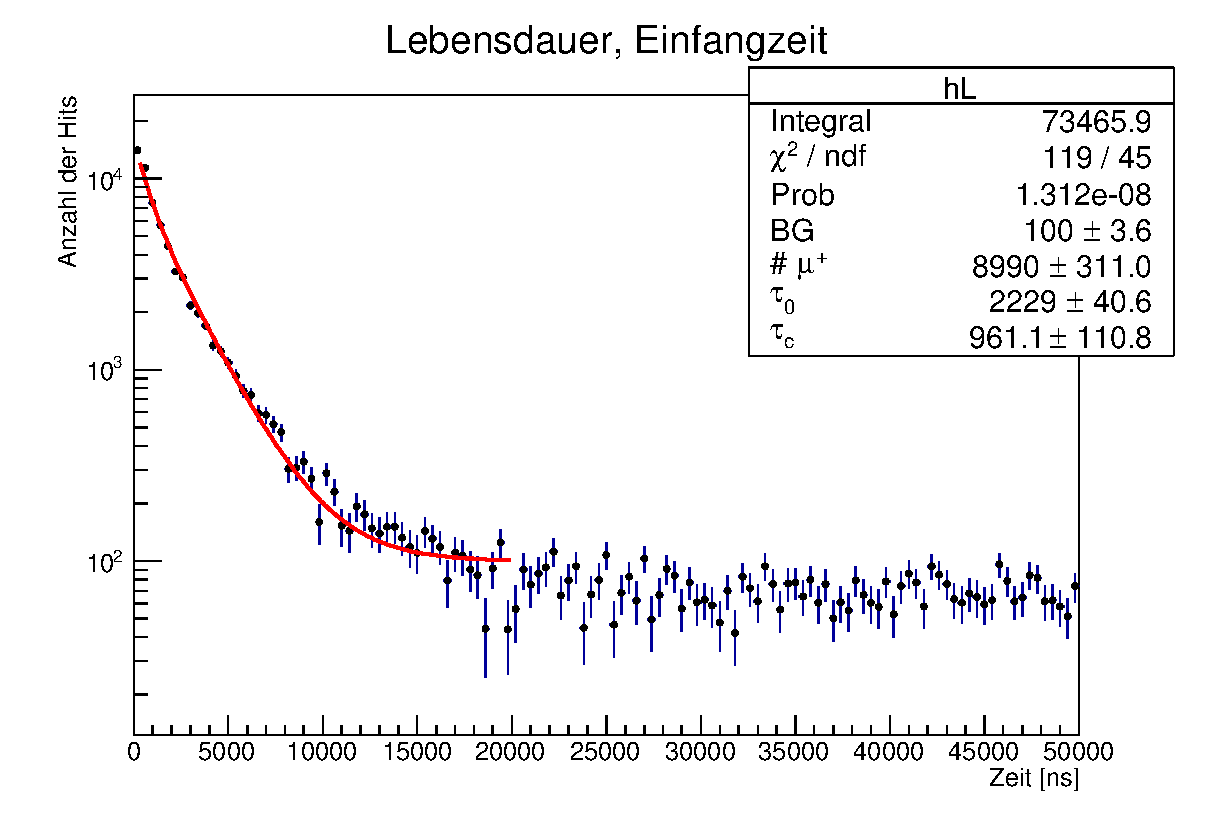
\includegraphics[width=120mm]{LebensdauerEinfangzeitKombiniert}
	\caption{ \itshape Nachpulskorrigiertes, kombiniertes Lebensdauerspektrum gefittet mit der Funktion \ref{eq:7}}
	\label{fig:Abbildung 2}
\end{figure}

\subsection{Bestimmung der Larmorfrequenz aus Messung mit Magnetfeld}
Wie im vorherigen Abschnitt wird wieder eine Nachpulskorrektur durchgeführt und Histogramme erstellt. Jedoch wird um die Daten zu fitten (Abbildung \ref{fig:Abbildung 3}
) eine Kombination des Histogramms ohne und mit Magnetfeld verwendet. Die jeweiligen Zählraten sind gegeben durch:

\begin{align}
\label{eq:12}
&Z^{with}(t)= Z_0 \cdot e^{-\frac{t}{\tau}} \cdot \left(
1 + P\cdot A \cdot
cos\left(\omega _{Larmor} t+\phi \right)
\right)\\
&Z^{without}(t)
= Z_0 \cdot e^{-\frac{t}{\tau}} \cdot \left(
1 + P\cdot A \cdot
cos\left(\phi \right)
\right)
\end{align}

\noindent Da die Messzeit mit und ohne Magnetfeld unterschiedlich war muss noch eine Skalierung $s = \frac{Z^{without} _0}{Z^{with} _0}$ berechnet werden. Das Histogramm wird dann mit folgender Funktion 
\begin{equation}
\label{eq:14}
\frac{Z^{without} (t)-Z^{with}(t)\cdot s}{Z^{without}(t)+Z^{with} (t) \cdot s} = \frac{P \cdot A}{2} \cdot
cos\left(
\omega_{Larmor} \cdot t
+
\phi
\right)
+
c
\end{equation}
bei festem $f=1.275 \pm 0.05$ gefittet. Die Abschätzung der systematischen Fehler erfolgt analog zum vorherigen Abschnitt. Durch Variation der Skalierungsfaktoren schätzen wir 
$\Delta \omega_{Larmor,sys} = 0.07 MHz$ und $\Delta PA_{sys} = 0.008$. Das Variieren der Fitrange um $\pm 10\%$ ergibt einen vernachlässigbaren statistischen Fehler von $\Delta \omega_{Larmor,sys,range} = 0.012 MHz$ und $\Delta PA_{sys,range} = 0.00038$.

\begin{figure}[h]
	\centering
	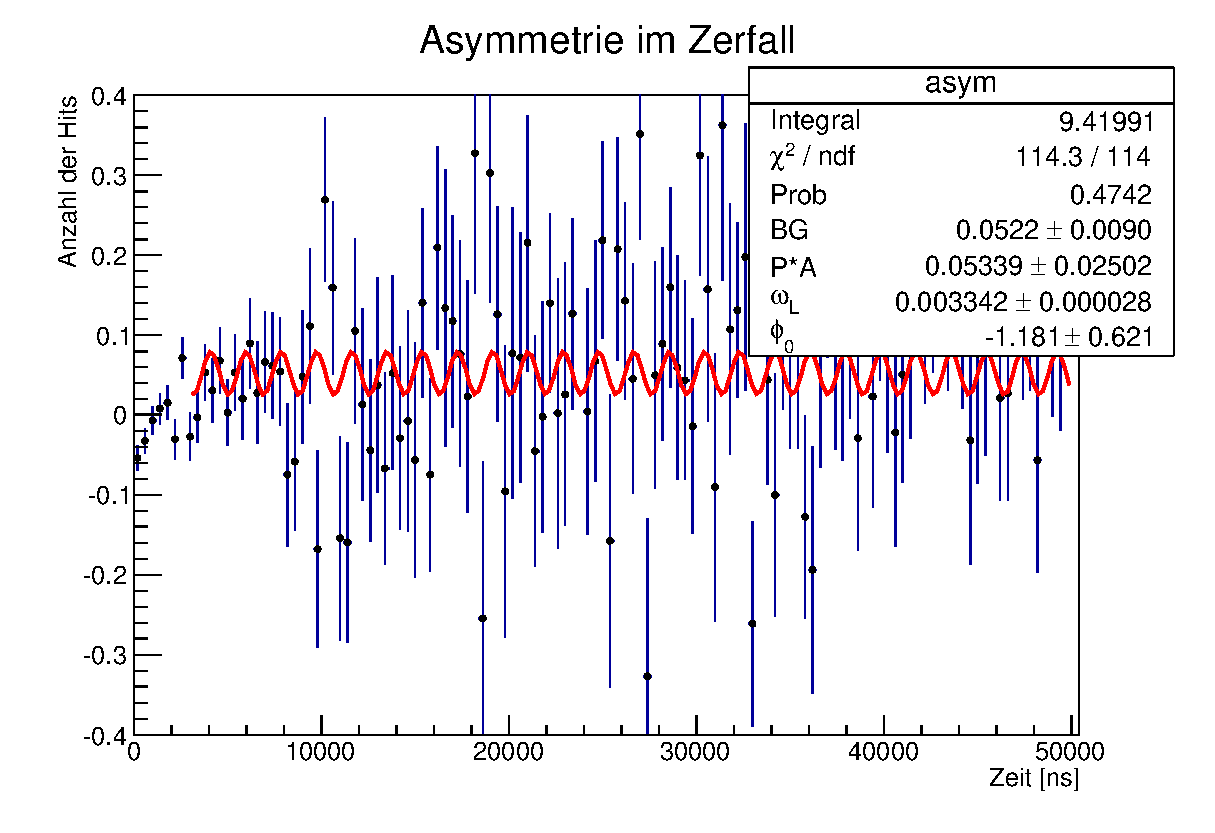
\includegraphics[width=120mm]{Asymmetrie}
	\caption{ \itshape Histogramm aus Messung mit Magnetfeld gefittet mit Funktion\ref{eq:14}}
	\label{fig:Abbildung 3}
\end{figure}
\noindent Als Ergebnis für die Larmorfrequenz erhalten wir also $\omega_{Larmor} = (3.342 \pm 0.028_{stat} \pm 0.041_{sys})\, MHz$. Mit diesem Wert berechnen wir nun das magnetische Moment des Myons nach (zur Berechnung wurden statistischer und systematischer Fehler addiert):
\begin{equation}
\mu _{\mu} = \frac{\hbar \cdot
 \omega_{Larmor}}{g\cdot B}
\end{equation}
Wir nehmen $g=2$ an da die Korrektur von $g$ deutlich kleiner als unser Messfehler ist. Damit erhält man $\mu_{\mu}  = (2.75  \pm 0.04)\times 10^{-7} eV \, T^{-1}$. Die Abweichung zum Literaturwert $\mu_{\mu, Lit} = 2,80 \times 10^{-11} eV \, T^{-1}$ liegt bei $1.25\sigma$ und somit sind die Werte miteinander vereinbar.
Aus dem Fitergebnis von $P\cdot A = 0.053\pm 0.025_{stat} \pm 0.008_{sys}$ kann man mit $A=0,23$ die Polarisation $P$ der Myonen bestimmen. Man erhält den Wert $P = 0.23 \pm 0.11_{stat} \pm 0.03_{sys}$. Dieser weicht somit mit einer Diskrepanz von $2\sigma$ nicht signifikant von $P=0$ ab. Die Messung weist also lediglich ein Indiz auf, dass die Myonen polarisiert sind und somit die Parität verletzt ist, aber man kann es mit diesem Wert nicht nachweisen. Mit dem erweiterten Datensatz anderer Gruppen erhalten wir analog $\mu_{\mu} = (2.87 \pm 0.04)\times 10^{-7} eV \, T^{-1}$ mit einer Diskrepanz von $1.75\sigma$ zum Literaturwert und $P = (0.1391 \pm 0.039_{stat} \pm 0.034_{sys})$ mit einer Diskrepanz zu $P=0$ von $2.7\sigma$.
\begin{figure}[h]
	\centering
	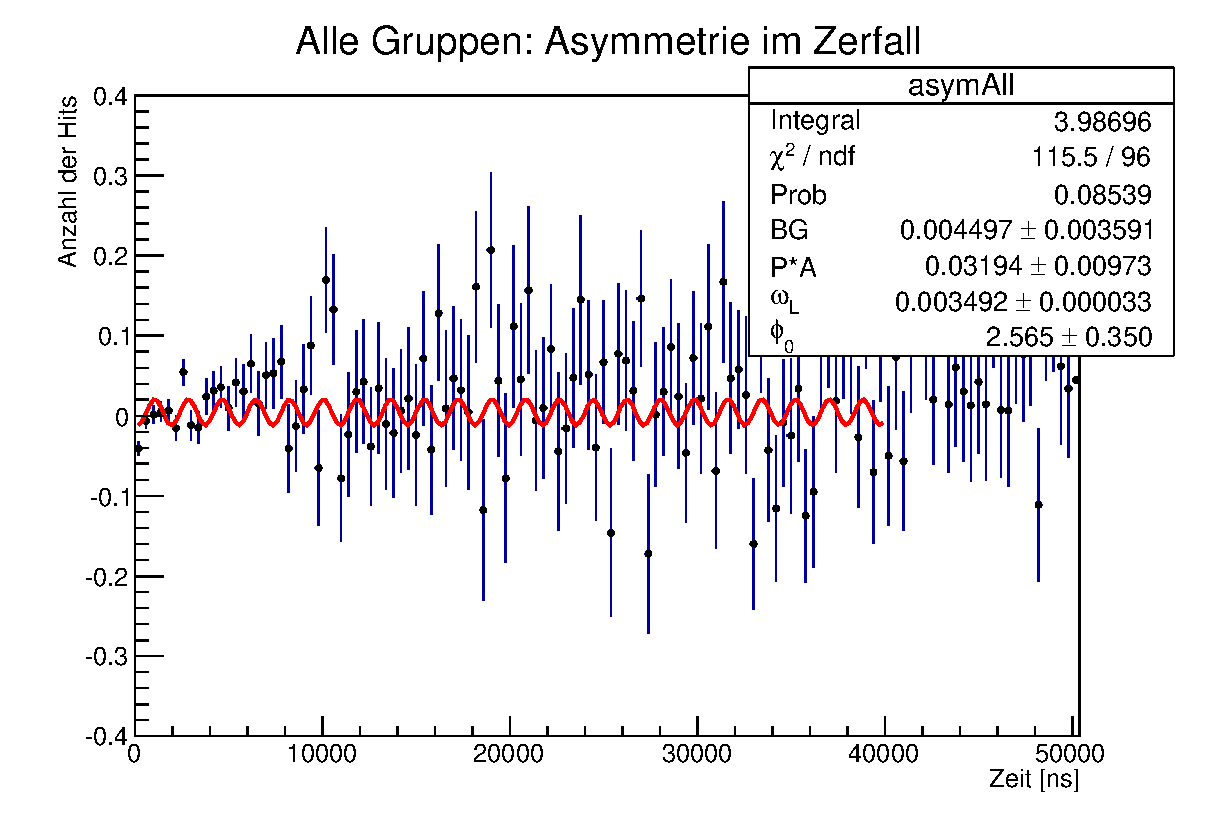
\includegraphics[width=120mm]{AlleGruppenAsymmetrie}
	\caption{ \itshape Histogramm aus Messung aller Gruppen mit Magnetfeld gefittet mit Funktion\ref{eq:14} }
	\label{fig:Abbildung 4}
\end{figure}
